\documentclass[11pt,a4paper]{article}
\usepackage[a4paper,margin=2.4cm]{geometry}
\usepackage{fontspec}
\usepackage{amsmath,amssymb,amsthm}
\usepackage{unicode-math}
\setmainfont{Liberation Serif}
\setsansfont{Liberation Sans}
\setmonofont{DejaVu Sans Mono}[Scale=0.82]
\setmathfont{Latin Modern Math}
\usepackage{polyglossia}
\setdefaultlanguage{russian}
\setotherlanguage{english}
\newfontfamily\cyrillicfont{Liberation Serif}
\newfontfamily\cyrillicfontsf{Liberation Sans}
\newfontfamily\cyrillicfonttt{DejaVu Sans Mono}[Scale=0.82]
\usepackage{booktabs,longtable,array}
\usepackage{enumitem}
\setlist{nosep,leftmargin=2em}
\usepackage[hidelinks]{hyperref}
\usepackage{microtype}
\usepackage{graphicx}

\theoremstyle{plain}
\newtheorem{theorem}{Теорема}[section]
\newtheorem{lemma}[theorem]{Лемма}
\newtheorem{proposition}[theorem]{Предложение}
\newtheorem{corollary}[theorem]{Следствие}
\theoremstyle{definition}
\newtheorem{definition}[theorem]{Определение}
\newtheorem{conjecture}{Гипотеза}
\newtheorem{problem}{Проблема}
\theoremstyle{remark}
\newtheorem*{remark}{Замечание}
\newtheorem*{example}{Пример}

\newcommand{\Z}{\mathbb{Z}}
\newcommand{\R}{\mathbb{R}}
\newcommand{\lc}{\ell_{\mathrm{cell}}}
\newcommand{\lseg}{\ell_{\mathrm{seg}}}
\newcommand{\lean}[1]{\texttt{#1}}
\DeclareMathOperator{\vol}{vol}

\title{\textbf{Относительная сетка}\\[4pt] \large Основной текст, версия 2.1}
\author{М.~Зафаров\thanks{Автор системы, определений и гипотез. Доказательства и текст оформлены с помощью ИИ-помощника Claude (Anthropic). Лицензия текста CC~BY~4.0, программ и файлов Lean — MIT. Репозиторий: \url{https://github.com/abema2416-ops/Relative-Grid}.}}
\date{28 ноября 2026 г.}

\begin{document}
\sloppy
\maketitle

\begin{abstract}
Это канонический текст системы «Относительная сетка». Он содержит только ядро системы, доказанные утверждения и явно помеченные гипотезы. Рабочий журнал (черновик 1.18, история версий, все проверки) и короткая статья (8 страниц) лежат в репозитории отдельно. Ядро — действия над конечными множествами клеток решётки $\Z^n$: растяжение и сжатие части объекта вдоль одной оси в целое число раз, удаление клеток, склеивание и расклеивание соседей по стороне. Изучаются две меры: потеря информации действия (в битах) и число действий, нужное для построения формы. Надстройки (повороты, тонкие объекты, склейки по ребру и вершине, исход совпадения) вынесены в приложение и помечены как эскизы.
\end{abstract}

\tableofcontents

\section{Введение и статус результатов}

\paragraph{Задача.} Фигура, нарезанная сеткой, — набор клеток. Мы задаём небольшой набор действий над такими наборами и спрашиваем: сколько действий нужно, чтобы построить данную форму из одной клетки, и сколько информации при этом теряется.

\paragraph{Что в системе своё.} Само действие $\alpha$ — частный случай аффинного растяжения (теорема~\ref{thm:affine}); подсчёт дыр опирается на клеточную гомологию; с растяжением и сжатием перекликаются дилатация и эрозия математической морфологии. Своё в системе: (1) способ задания действия — зона и закреплённая сторона в клетках; (2) потеря в битах для действий над формами и асимметрия «убрать дорого, вернуть бесплатно»; (3) склейки, отделённые от касаний, и их связь с числом дыр; (4) число действий $\ell$, его NP-трудность для рельефов, вычислимость без потерь и правило отрезков. Сравнение с близкими работами — в §\ref{sec:related}.

\paragraph{Как помечены результаты.} В таблице~\ref{tab:status} для каждого результата указано, чем он подтверждён: \textbf{L} — доказан машинно в Lean~4 (только стандартные аксиомы, без пропусков); \textbf{L+T} — главная часть в Lean, остальное — строгим текстом; \textbf{T} — строгое доказательство в тексте; \textbf{K} — опирается на опубликованную теорему; \textbf{П} — только проверка перебором (не доказательство).

\begin{longtable}{p{0.47\textwidth}cp{0.36\textwidth}}
\caption{Статус результатов}\label{tab:status}\\
\toprule
Результат & Статус & Где\\
\midrule
\endfirsthead
\toprule Результат & Статус & Где\\ \midrule \endhead
Свойства $\alpha$: число клеток, нет наложений, слияние в блоке & L & §\ref{sec:props}\\
Растяжение без потерь; прообразы $\sigma$ & L & §\ref{sec:props}\\
Сдвиг объекта вместе с зоной & L & §\ref{sec:shift}\\
Каждая исчезнувшая клетка стоит $\ge1$ бита & L+T & §\ref{sec:loss}\\
Потеря $\ge|A|-|B|$; убрать $h$ бит, вернуть 0 & L+T & §\ref{sec:loss}\\
Точная потеря сжатия ряда & T + П & §\ref{sec:loss}\\
Растяжение = аффинное растяжение & L & §\ref{sec:affine}\\
Пределы конечных цепочек (растяжения, сжатия, $\sigma$) & T & §\ref{sec:affine}\\
Склейки и дыры на плоскости & L+T & §\ref{sec:holes}\\
$m(O)\le\lc(O)\le|O|-1$; брусок за $k$ действий & L+T & §\ref{sec:count}\\
$\lc\le\ell\le\lc+2$; рамка $+\sigma$ за $n+1$ & T & §\ref{sec:count}\\
Вычислимость $\ell$ без потерь & L+T & §\ref{sec:count}\\
Рельефы: $R(H)$ и нормальный базис, NP-трудность & L+T+K & §\ref{sec:reliefs}\\
Оценки и точные случаи $R(H)$ & L & §\ref{sec:reliefs}\\
Ранговая граница $R\ge\operatorname{rank}A$ & T & §\ref{sec:reliefs}\\
Метод деревьев (где прячется экономия) & T & §\ref{sec:reliefs}\\
Вычислительный метод: 30/30 трудных задач, задачи на 150--257 высот & П & §\ref{sec:compute}\\
Правило отрезков: $\lseg\ge\ell_\alpha$; равенство при $\ell_\alpha\le2$ & T & §\ref{sec:seg}\\
Правило отрезков в общем случае & П & §\ref{sec:seg}, гипотеза~\ref{conj:seg}\\
Нижняя граница для рельефов & T (модель) / П & §\ref{sec:reliefs}, гипотеза~\ref{conj:relief}\\
\bottomrule
\end{longtable}

\section{Ядро системы}\label{sec:core}

\subsection{Клетки, объекты, формы}

Обозначения: $e_1,\dots,e_n$ — единичные векторы осей; $|X|$ — число элементов; $\|v\|_1=\sum|v_i|$; $c[i\mapsto v]$ — клетка $c$ с заменённой $i$-й координатой.

\begin{definition}
\emph{Клетка} — точка $c\in\Z^n$; она изображает куб $Q(c)=c+[0,1]^n$. Клетки $c,c'$ — \emph{соседи по стороне}, если $\|c-c'\|_1=1$. \emph{Объект} — пара $(O,S)$: $O\subset\Z^n$ конечно и непусто, $S$ — множество \emph{склеек}, то есть неупорядоченных пар соседей по стороне из $O$. Соседи без склейки образуют \emph{трещину}. \emph{Кусок} — компонента связности графа склеек. \emph{Форма} — класс $[O]=\{O+v: v\in\Z^n\}$.
\end{definition}

\subsection{Действия}\label{sec:actions}

\begin{definition}[растяжение и сжатие]\label{def:alpha}
Параметры: конечная зона $Z\subset\Z^n$, ось $i$, направление $s\in\{\pm1\}$, коэффициент $f\ge2$. Пусть $G=O\cap Z\ne\varnothing$, $a=\min\{sc_i:c\in G\}$ (закреплённая сторона), $t(c)=sc_i-a$. Тогда
\begin{align*}
\alpha^{\uparrow}(O)&=(O\setminus G)\cup\{c[i\mapsto s(a+f\,t(c)+j)]: c\in G,\ 0\le j<f\},\\
\alpha^{\downarrow}(O)&=(O\setminus G)\cup\{c[i\mapsto s(a+\lfloor t(c)/f\rfloor)]: c\in G\}.
\end{align*}
\textbf{П3.} Действие допустимо, только если новые клетки не задевают $O\setminus G$; иначе оно отклоняется (параметра, разрешающего совпадения, в ядре нет).
\textbf{Склейки.} При растяжении $f$ клеток образа одной клетки склеены подряд, а склейка $\{c,c'\}$ переходит в склейки всех пар их образов, соседних по стороне. При сжатии склейка переходит в склейку образов; если клетки слились, она исчезает.
\textbf{П5.} Действие, после которого склеенные клетки перестали бы быть соседями по стороне, недопустимо.
\end{definition}

\begin{definition}[$\sigma$, $\beta_\pm$]
$\sigma_Z(O)=O\setminus Z$ (склейки удалённых клеток исчезают). $\beta_+(K)$ добавляет к $S$ непустое множество $K$ несклеенных соседних пар; $\beta_-(K')$ удаляет непустое $K'\subset S$. Одно применение $\beta$ — одно действие, сколько бы пар ни было в $K$.
\end{definition}

\subsection{Потеря и число действий}

\begin{definition}[потеря]
Действие $\varphi$ с фиксированными $(Z,i,s,f)$ применимо к любому содержимому зоны. Потеря считается по клеткам:
\[
\lambda(\varphi,O)=\log_2\bigl|\{O'\subset\Z^n:\ O'\setminus Z=O\setminus Z,\ \varphi\text{ допустимо на }O',\ \varphi(O')=\varphi(O)\}\bigr|.
\]
Потеря цепочки — сумма потерь шагов. $\lambda(\beta_\pm)=0$: клетки не меняются, а по паре $(O,S)$ при известном $K$ прообраз единственен — $(O,S\setminus K)$ для $\beta_+(K)$ и $(O,S\cup K)$ для $\beta_-(K)$.
\end{definition}

\begin{definition}[число действий]
Цепочка начинается с одной клетки без склеек. Для набора действий $\mathcal A\subset\{\alpha^\uparrow,\alpha^\downarrow,\sigma,\beta_+,\beta_-\}$:
$\lc^{\mathcal A}(O)$ — наименьшая длина цепочки из $\mathcal A$, после которой множество клеток равно $O$ (склейки любые);
$\ell^{\mathcal A}(O,S)$ — то же со склейками ровно $S$.
Без индекса берётся всё ядро; $\ell_\alpha=\lc^{\{\alpha^\uparrow\}}$. \emph{Стоимость склеек} — число пар, склеенных действиями $\beta_+$; в $\ell$ она не входит.
\end{definition}

\subsection{Сдвиг и зоны}\label{sec:shift}

Зоны задаются в координатах конкретного представителя формы. Сдвиг объекта на $v$ сопровождается сдвигом зоны.

\begin{proposition}[\lean{stretch\_shift}, \lean{shrink\_shift}, \lean{sigma\_shift}, \lean{anchor\_shift}]
$\alpha_{Z+v}(O+v)=\alpha_Z(O)+v$ (для растяжения и сжатия; закреплённая сторона переходит в $a+sv_i$) и $\sigma_{Z+v}(O+v)=\sigma_Z(O)+v$. Следовательно, цепочку можно сдвинуть целиком вместе с зонами; $\ell$ и $\lambda$ не зависят от выбора представителя и начальной клетки.
\end{proposition}

Зона, не сдвинутая вместе с объектом, задаёт другое действие: в общем случае $\alpha_Z(O+v)\neq\alpha_Z(O)+v$.

\section{Основные свойства действий}\label{sec:props}

\begin{proposition}\label{prop:basic}
\begin{enumerate}[label=\upshape(\alph*)]
\item Клетки вне зоны не меняются; у образов не меняются координаты, кроме $i$-й (\lean{stretch\_keeps\_rest}, \lean{img\_r}).
\item При допустимом растяжении образы разных клеток не пересекаются и $|\alpha^\uparrow(O)|=|O|+(f-1)|G|$ (\lean{stretch\_card}, \lean{img\_inj}).
\item При сжатии две клетки сливаются тогда и только тогда, когда они в одном ряду и $\lfloor t/f\rfloor$ совпадает (\lean{shrink\_merge}, \lean{shrinkCell\_eq\_iff}).
\item Растяжение без потерь: два содержимых зоны с одинаковым результатом совпадают (\lean{stretch\_lossless}).
\item $\sigma_Z(O')=\sigma_Z(O)$ тогда и только тогда, когда $O'$ и $O$ совпадают вне $Z$; поэтому $\lambda(\sigma_Z)=|Z|$ (\lean{sigma\_preimage}).
\end{enumerate}
\end{proposition}

\begin{proposition}[что не меняет каждое действие ядра]
\begin{center}
\begin{tabular}{lccc}
\toprule
& клетки & куски & дыры $d$ ($n=2$)\\
\midrule
$\alpha^\uparrow$ & $+$ & не меняет & не меняет\\
$\alpha^\downarrow$ & $-$ & может & может\\
$\beta_+$ & не меняет & $-1$ или $0$ & $+1,0,-1$\\
$\beta_-$ & не меняет & $+1$ или $0$ & $+1,0,-1$\\
$\sigma$ & $-$ & может & может\\
\bottomrule
\end{tabular}
\end{center}
\end{proposition}
\begin{proof}
Растяжение: склейки переходят в склейки, новых склеек между кусками нет, по П5 рвать нельзя; дыры — теорема~\ref{thm:holes}(b). Склейка соединяет две клетки одного или двух кусков. Сжатие и $\sigma$ — примеры: две несклеенные соседние клетки, сжатые вдвое, дают одну; кольцо $3\times3$, сжатое втрое вдоль ряда, теряет дыру.
\end{proof}

\section{Потеря информации}\label{sec:loss}

\begin{lemma}\label{lem:bit}
Если действие уменьшает число клеток на $d>0$, то его потеря не меньше $d$ бит.
\end{lemma}
\begin{proof}
Для $\sigma$ — предложение~\ref{prop:basic}(e). Пусть действие — сжатие; непустые блоки $B_0$ (содержит клетку $e$, на которой достигается $a$), $B_1,\dots,B_r$, в блоке $B$ — $m_B$ клеток группы, $d=\sum(m_B-1)$. Рассмотрим объекты $O'$, совпадающие с $O$ вне $Z$, у которых $O'\cap Z\subset G$, $e\in O'$ и каждый $B_k$ непуст. (1) Закреплённая сторона та же (\lean{anchor\_of\_subset}). (2) Результат тот же (\lean{shrink\_same\_of\_blocks}). (3) Новые клетки — часть прежних, поэтому П3 выполняется. (4) Выборы в разных блоках независимы: в $B_0$ клетка $e$ обязательна ($2^{m_{B_0}-1}$ вариантов), в $B_k$ — любое непустое подмножество ($2^{m_{B_k}}-1$). (5) $2^{m_0-1}\prod(2^{m_k}-1)\ge2^d$ (\lean{loss\_ge\_bits\_anchor}).
\end{proof}

\begin{theorem}\label{thm:loss}
(a) При любом превращении $A\to B$ потеря не меньше $|A|-|B|$ бит. (b) Если $A$ связен по сторонам, $B=A\setminus H\ne\varnothing$, $|H|=h$, то наименьшая потеря $A\to B$ равна $h$ бит, а $B\to A$ — нулю. (c) Для связного по сторонам $B$ наименьшая потеря $A\to B$ лежит между $\max(0,|A|-|B|)$ и $|A|-1$.
\end{theorem}
\begin{proof}
(a) Суммируем лемму~\ref{lem:bit} по шагам. (b) $h$ достигается $\sigma_H$. Обратно: каждая компонента $H$ граничит по стороне с $B$, клетки $H$ упорядочиваются так, что каждая — сосед уже построенной; каждую возвращает растяжение соседа вдвое в её сторону (\lean{grow\_one}), без потерь (\lean{stretch\_lossless}). (c) Сверху: $\sigma$ оставляет одну клетку ($|A|-1$ бит), затем рост без потерь (теорема~\ref{thm:bounds}).
\end{proof}

\begin{theorem}[точная потеря сжатия ряда]\label{thm:exact}
Пусть зона — отрезок ряда с позициями $0,\dots,L-1$, $a$ — наименьшая занятая позиция, ряд сжимается в $f$ раз; позиции $a,\dots,L-1$ делятся на блоки по $\lfloor(p-a)/f\rfloor$, $z_B$ — число позиций зоны в блоке $B$, $B_0$ — блок якоря. Тогда число содержимых зоны с тем же результатом равно
\[
N=2^{\,z_{B_0}-1}\prod_{B\ne B_0,\ B\text{ непуст}}\bigl(2^{z_B}-1\bigr).
\]
\end{theorem}
\begin{proof}
Результат определяется якорем и множеством непустых блоков. Содержимое даёт тот же результат ровно тогда, когда его самая левая клетка — $a$ и непусты те же блоки. Выборы в блоках независимы.
\end{proof}
Проверено полным перебором на 2872 случайных рядах ($L\le13$, $f=2,3,4$). Пример: $L=20$, $f=2$, исчезло 4 клетки — лемма даёт $N\ge16$, теорема $N=4374$.

\begin{example}
Ряд из 4 клеток $\{0,1,2,3\}$ сжимается вдвое: блоки $\{0,1\}$ и $\{2,3\}$, результат $\{0,1\}$. Прообразы: клетка $0$ обязательна, клетка $1$ любая ($2$ варианта), из $\{2,3\}$ — любое непустое подмножество ($3$ варианта); $N=6$, потеря $\log_2 6\approx2{,}58$ бита при двух исчезнувших клетках.
\end{example}

\begin{figure}[h]\centering
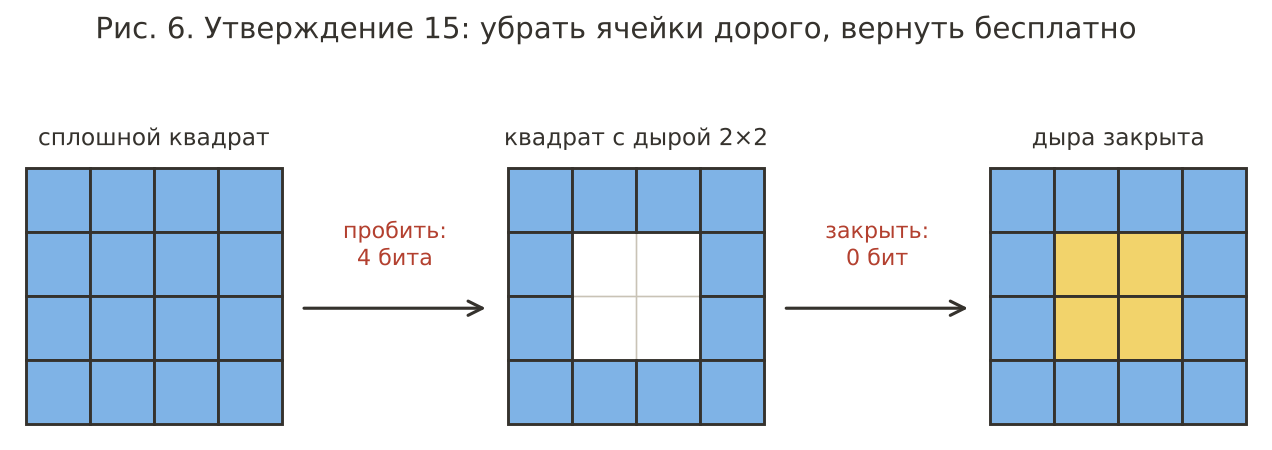
\includegraphics[width=0.8\textwidth]{fig6.png}
\caption{Теорема~\ref{thm:loss}(b): пробить дыру из 4 клеток стоит 4 бита, закрыть — 0 бит.}
\end{figure}

\section{Связь с непрерывной геометрией}\label{sec:affine}

Пусть $F(O)=\bigcup_{c\in O}Q(c)$, $y=sx_i$, $T\colon y\mapsto a+f(y-a)$.

\begin{theorem}\label{thm:affine}
(a) $F(\alpha^\uparrow(O))=F(O\setminus G)\cup T(F(G))$ точно (\lean{T\_cell}, \lean{block\_eq\_cells}). (b) $\alpha^\downarrow(O)=(O\setminus G)\cup\{c:\vol(Q(c)\cap T^{-1}F(G))>0\}$ (\lean{shrink\_slab}).
\end{theorem}
\begin{proof}
(a) Клетка с позицией $p=a+t$ переходит в клетки $a+ft,\dots,a+ft+f-1$, занимающие $T([p,p+1))$. (b) $T^{-1}$ переводит клетку в слой толщины $1/f$ внутри клетки $a+\lfloor t/f\rfloor$.
\end{proof}

\begin{figure}[h]\centering
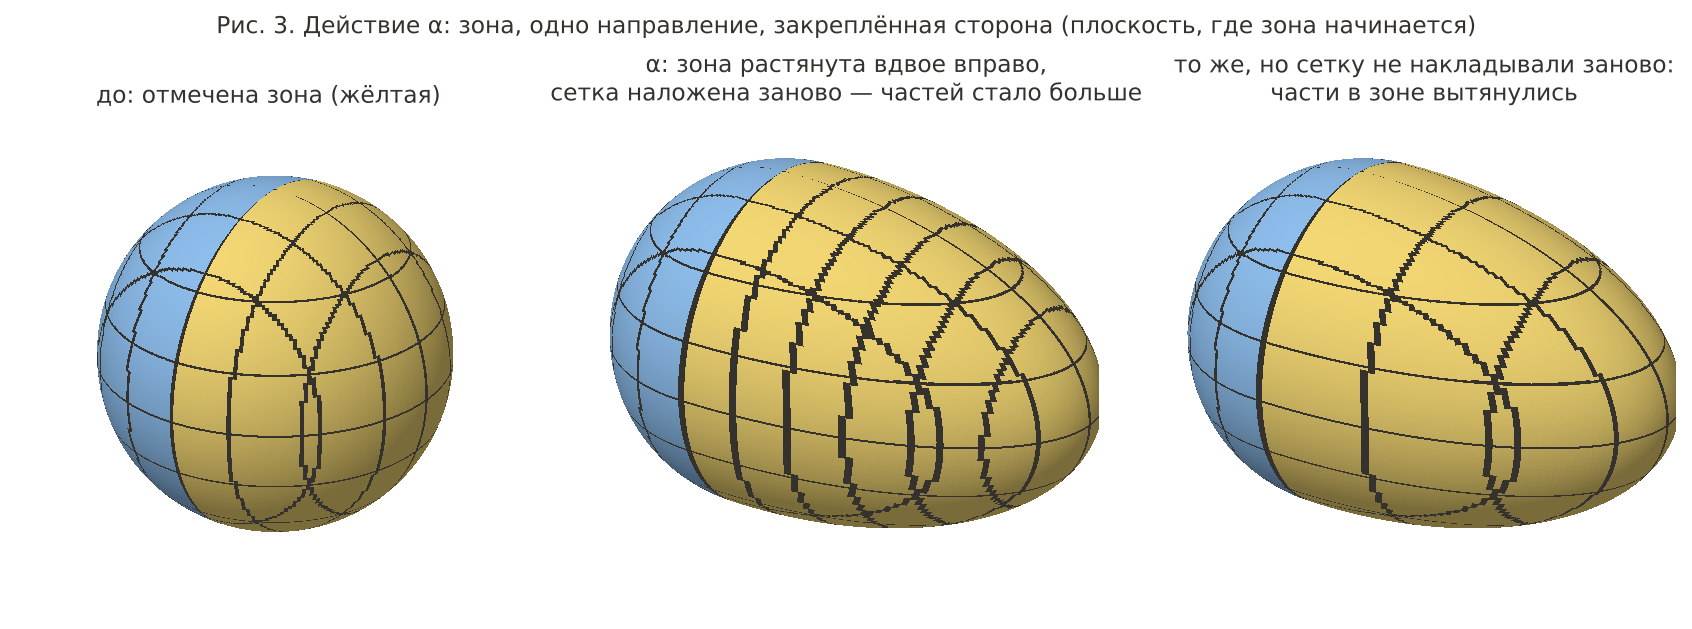
\includegraphics[width=0.9\textwidth]{fig3.png}
\caption{Действие $\alpha$ на шаре: зона растянута вдвое от закреплённой стороны. Слева направо: зона отмечена; растянуто и снова нарезано сеткой; то же без повторной нарезки. По теореме~\ref{thm:affine} обе картины изображают одну и ту же фигуру $T(F(G))$.}
\end{figure}

\paragraph{Пределы.} Запись фигуры $F$ на уровне $N$ — множество клеток уровня $N$, в которых $F$ занимает долю не меньше порога $\theta\in(0,1]$ (или положительную долю при $\theta=0^+$).

\begin{theorem}[записи одной фигуры]\label{thm:rec}
Если $F$ ограничена и измерима по Жордану, то записи $F$ сходятся к $F$ по объёму, а их округления на каждом фиксированном уровне стабилизируются при $\theta=0^+$ всегда и при $\theta\in(0,1]$ — для всех порогов, кроме не более чем счётного множества.
\end{theorem}
\begin{proof}
Ошибочные клетки задевают $\partial F$, а их суммарный объём стремится к нулю. Доля записи в каждой клетке крупного уровня сходится к доле $F$; округление стабилизируется, если эта доля не равна $\theta$. Пар (уровень, клетка) счётное число.
\end{proof}

\begin{theorem}[конечные цепочки]\label{thm:limit}
Пусть на уровнях $N_1\mid N_2\mid\cdots$ записи $O_N$ и группы $G_N$ сходятся по объёму к ограниченным $F\supset K$, $K$ измеримо по Жордану, якоря $a_N/N\to A$. Тогда растяжения $\alpha^\uparrow(O_N)$ сходятся к $(F\setminus K)\cup T_A(K)$, сжатия $\alpha^\downarrow(O_N)$ — к $(F\setminus K)\cup T_A^{-1}(K)$, а $\sigma_{Z_N}(O_N)$ при $F(O_N\cap Z_N)\to W$ — к $F\setminus W$. То же для любой конечной цепочки, если пределы групп всех сжатий измеримы по Жордану.
\end{theorem}
\begin{proof}
Растяжение: по теореме~\ref{thm:affine}(a); $T$ умножает объём на $f$, малый сдвиг якоря даёт малую ошибку. Сжатие: пусть $B(X)$ — сжатие множества клеток $X$ с якорем $a_N$, $K_N$ — запись $K$. (1) $|B(G_N)\triangle B(K_N)|\le|G_N\triangle K_N|$: блок из разности содержит клетку из разности, разные блоки — разные клетки. (2) $F(B(K_N))\supseteq T^{-1}F(K_N)$; лишний объём дают только неполные блоки, в каждом есть соседние клетки из $K_N$ и не из $K_N$, их объединение задевает $\partial K$, а таких клеток $o(N^n)$. (3) $\vol(T^{-1}F(K_N)\triangle T^{-1}K)=\vol(F(K_N)\triangle K)/f\to0$. Объединения и разности — неравенством для симметрической разности.
\end{proof}

\section{Склейки и дыры на плоскости}\label{sec:holes}

Пусть $n=2$. Комплекс $K(O,S)$: по квадрату на клетку, общие стороны склеенных пар отождествлены. Число дыр $d=\dim H_1(K;\mathbb Q)$; $q$ — число точек решётки, окружённых целиком склеенным квадратом $2\times2$.

\begin{theorem}\label{thm:holes}
(a) $d=(\text{число кусков})-|O|+|S|-q$. (b) Допустимое растяжение не меняет $d$. (c) Одна склейка меняет $d$ на $+1$, $0$ или $-1$. (d) Чтобы построить объект растяжениями и склейками, нужно склеить не меньше $d$ пар; при $q=0$ ровно $d$ пар достаточно.
\end{theorem}
\begin{proof}
(a) Граней $|O|$, рёбер $4|O|-|S|$. Над точкой $p$ граф $\Gamma(p)$ (квадраты с углом $p$; склеенные стороны с концом $p$) — подграф 4-цикла; число вершин $K$ над $p$ равно числу его компонент $k-s+[\text{цикл}]$ (\lean{vertex\_count}). Отсюда $\chi=|O|-|S|+q$ (\lean{euler}). По теореме о ранге $\chi=b_0-b_1+b_2$. $b_2=0$: в ненулевом 2-цикле возьмём квадрат с ненулевым коэффициентом и лексикографически наибольшей клеткой; его правая сторона общая только с квадратом справа, коэффициент которого $0$, — противоречие. Компоненты $K$ — куски.
(b) Клеток $+(f-1)|G|$, склеек $+(f-1)|G|+(f-1)r$ ($r$ — склейки внутри $G$ поперёк оси), $q$ растёт на $(f-1)r$, куски не меняются (\lean{stretch\_keeps\_d}). (c) Склейка внутри куска: $|S|+1$, $q+\{0,1,2\}$; между кусками: кусков на 1 меньше, $q$ не меняется (\lean{glue\_inside}, \lean{glue\_join}, \lean{three\_seams\_connect}). (d) Из (b), (c) (\lean{d\_le\_glues}); сверху — рост по остовному дереву графа склеек и $|S|-|O|+1$ склеек.
\end{proof}

Следствие: у дыры два способа появиться — склейкой (0 бит) или пробиванием (не меньше бита на клетку).

\begin{figure}[h]\centering
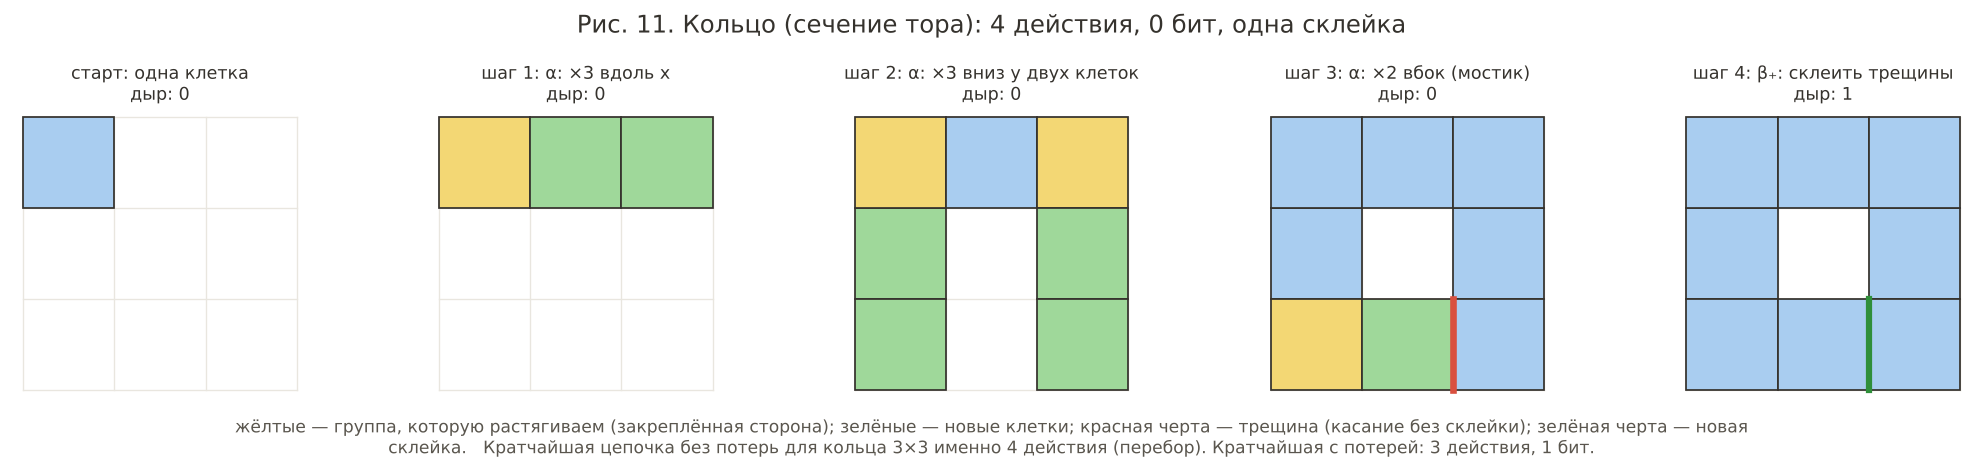
\includegraphics[width=\textwidth]{fig11a.png}
\caption{Кольцо $3\times3$ без потерь: три растяжения и одна склейка. Растяжения не создают дыру (теорема~\ref{thm:holes}(b)); её замыкает склейка трещины. С потерей кольцо строится за 3 действия (квадрат $3\times3$ и $\sigma$ центра, 1 бит).}
\end{figure}

\begin{example}
Кольцо $3\times3$, все 8 стыков склеены: $d=1-8+8-0=1$. Без одного стыка: $d=0$ (в кольце трещина). Квадрат $2\times2$, все стыки склеены: $d=1-4+4-1=0$. Квадрат $2\times3$ без среднего внутреннего стыка: $d=1-6+6-0=1$ — внутренняя трещина считается дырой.
\end{example}

\begin{theorem}[дыра без потерь требует склейки]
Пусть цепочка из одной клетки строит объект с $d\ge1$. Тогда в ней есть $\beta_+$, $\beta_-$, $\sigma$, убирающее клетку, или сжатие со слиянием.
\end{theorem}
\begin{proof}
Растяжения не меняют $d$; сжатие без слияния — изоморфизм графов склеек, сохраняющий целиком склеенные квадраты, поэтому тоже не меняет $d$. У одной клетки $d=0$.
\end{proof}

\section{Число действий}\label{sec:count}

Пусть $m(O)$ — число осей, вдоль которых у клеток $O$ есть два разных значения координаты.

\begin{theorem}\label{thm:bounds}
(a) $m(O)\le\lc(O)$ для любого объекта и любой цепочки ядра (\lean{axes\_le\_length}). (b) Если $O$ связен по сторонам, то $\ell_\alpha(O)\le|O|-1$, и цепочка без потерь. (c) Брусок со сторонами $\ge2$ по $k$ осям: $\lc=k$, и с всеми склейками соседей тоже $k$. (d) $\lc(O)\le\ell(O,S)\le\lc(O)+2$. (e) Если разрешено $\sigma$, то $\lc(O)\le n+1$ для любого $O$, и такая цепочка теряет $|P|-|O|$ бит ($P$ — наименьший брусок, содержащий $O$).
\end{theorem}
\begin{proof}
(a) Значения $i$-й координаты растут только при $\alpha$ вдоль оси $i$; формально — \lean{step\_spreads}, \lean{chain\_spreads}. (b) Обход в ширину по графу соседства; каждый шаг — \lean{grow\_one}. (c) По оси растяжение на каждую; растяжения сами склеивают всех соседей по стороне. (d) Добавить в конце $\beta_-(S'\setminus S)$ и $\beta_+(S\setminus S')$. (e) Рамка за $\le n$ растяжений и $\sigma_{P\setminus O}$ с $2^{|P\setminus O|}$ прообразами.
\end{proof}

\begin{example}
Куб $m\times m\times m$ из одной клетки: растяжение в $m$ раз по каждой оси, $\lc=3$ при любом $m\ge2$ (меньше нельзя по (a)). Буква «Г» из 5 клеток на плоскости: ряд из 3 клеток, затем крайняя клетка вверх в 3 раза — 2 действия, $m=2$, оценка (a) точна. Кольцо $3\times3$: $\ell_\alpha=3$, но для кольца со склеенными стыками нужно ещё $\beta_+$ (рис. 3), $\ell=4$; с $\sigma$ — 3 действия и 1 бит.
\end{example}

Пункт (e) — обмен работы на потерю: любая форма за $n+1$ действий, но с битами за каждую вырезанную клетку.

\begin{theorem}[вычислимость без потерь]\label{thm:dec}
Для $\mathcal A=\{\alpha^\uparrow\}$ и $\mathcal A=\{\alpha^\uparrow,\beta_\pm\}$ числа $\lc^{\mathcal A}(O)$ и $\ell^{\mathcal A}(O,S)$ вычислимы.
\end{theorem}
\begin{proof}
(1) Рамка при растяжении не сужается, поэтому все промежуточные фигуры лежат в рамке итоговой (\lean{stretch\_frame}, \lean{schain\_frame}). (2) Число клеток не убывает (\lean{stretch\_card}). (3) Коэффициент не больше стороны рамки (\lean{stretch\_image\_ends}). (4) Результат зависит лишь от $G=O\cap Z$, оси, направления и $f$. Значит, состояний и переходов конечно много, поиск в ширину завершается.
\end{proof}

Следствие: все переборы в ограниченных коробках в §\ref{sec:seg} точны. При разрешённых сжатиях и $\sigma$ фигура может выйти за рамку, и вопрос открыт (проблема~\ref{pr:dec}).

\section{Рельефы и трудность счёта}\label{sec:reliefs}

Рельеф: основание $B\subset\Z^{n-1}$, высоты $h\colon B\to\{1,2,\dots\}$, $O=\{(b,j):0\le j<h(b)\}$. В \emph{модели столбиков} сначала строится основание, затем растягиваются вверх зоны из целых столбиков; высота — произведение коэффициентов. $H$ — множество высот больше 1, $D=|H|$, $R(H)$ — наименьшее число множителей, из подмножеств которых собираются все высоты. Тогда $\ell(O)\le\ell(B)+R(H)$.

\begin{theorem}[кандидаты]\label{thm:cand}
Существует наименьший набор множителей из $C(H)=H\cup\mathcal D\cup\mathcal Q$, где $\mathcal D$ — числа $\ge2$, делящие две высоты, $\mathcal Q=\{h/d\ge2: d\in\mathcal D,\ d\mid h\}$.
\end{theorem}
\begin{proof}
Общий для двух высот множитель лежит в $\mathcal D$. У высоты не больше одного личного множителя (два заменяются произведением, \lean{step2}). Личный множитель высоты $h$ заменяется на $h/a$ при общем множителе $a$ в разложении $h$ (\lean{step3}), иначе на $h$.
\end{proof}

\begin{theorem}\label{thm:R}
(a) $\lceil\log_2(D+1)\rceil\le R\le D$ (\lean{card\_le\_pow}). (b) Попарно взаимно простые высоты: $R=D$ (\lean{coprime\_R\_eq\_D}). (c) $H=\{b,\dots,b^D\}$: $R=\lceil\log_2(D+1)\rceil$ (\lean{ladder\_exact}). (d) При фиксированном $k$ условие $R\le k$ проверяется за время, полиномиальное от $D$ и наибольшей высоты.
\end{theorem}
\begin{proof}
(a) $R$ множителей дают $\le2^R-1$ непустых частей. (b) Общий множитель делил бы обе высоты. (c) Двоичная запись показателя. (d) Перебор наборов из $k$ кандидатов теоремы~\ref{thm:cand}.
\end{proof}

\begin{theorem}[NP-трудность]\label{thm:np}
Для бесквадратных высот $R(H)$ равно наименьшему размеру нормального базиса семейства множеств простых делителей высот. Поэтому задача «$R(H)\le K$?» NP-трудна при двоичной записи высот.
\end{theorem}
\begin{proof}
Части разложения бесквадратной высоты свободны от квадратов и попарно не имеют общих делителей больше 1 (\lean{sqfree\_dvd}, \lean{sqfree\_parts\_disjoint}), поэтому их множества простых не пересекаются. Обратно, базису отвечают произведения простых. Семейство подмножеств $\{u_1,\dots,u_k\}$ кодируется первыми $k$ простыми; запись высот полиномиальна. Нормальный базис NP-полон \cite{jiang}.
\end{proof}

\paragraph{Таблица показателей.} Пусть $A$ — таблица: строка — высота, столбец — простое число, в клетке — показатель простого в высоте. Множитель — «прямоугольник» в этой таблице: высоты, которые его используют, $\times$ его показатели.

\begin{theorem}[ранговая граница]\label{thm:rank}
$R(H)\ge\operatorname{rank}_{\mathbb Q}A$.
\end{theorem}
\begin{proof}
Если высоты собираются из множителей $m_1,\dots,m_R$, то вектор показателей высоты $h$ равен $\sum_{m\in S_h}v(m)$. Значит, $A=UV$, где $U$ — таблица $0/1$ размера $|H|\times R$, а $V$ — таблица показателей множителей. Ранг произведения не больше $R$.
\end{proof}

Нижняя граница берётся как $\max(\operatorname{rank}A,\lceil\log_2(D+1)\rceil)$: логарифм силён, когда высот много, а ранг — когда много простых. Если она совпала с какой-нибудь верхней оценкой ($D$, число простых, ответ любого эвристического метода), ответ точный без перебора.

\begin{theorem}[где прячется экономия]\label{thm:tree}
Пусть набор $B$ собирает $H$; множитель назовём общим, если он входит в разложения хотя бы двух высот, и личным иначе; $T$ — высоты, разложенные только по общим. Тогда $|B|\ge(\text{число общих})+(|H|-|T|)$, и каждый множитель в разложении $h\in T$ лежит в $h\cap g$ для некоторой другой высоты $g$. Если $R(H)<|H|$, то найдётся группа $T$ с $R(T)<|T|$; её строки в $A$ линейно зависимы. Если у $A$ ровно одна зависимость строк, то $T$ содержит её носитель.
\end{theorem}
\begin{proof}
Каждая высота вне $T$ использует хотя бы один личный множитель, а личные у разных высот разные. Общий множитель, входящий в $h$ и в $g$, лежит в $h\cap g$. Из $R(T)<|T|$ и теоремы~\ref{thm:rank} следует $\operatorname{rank}(T)<|T|$; зависимость строк $T$ продолжается нулями до зависимости строк $H$, то есть кратна единственной.
\end{proof}

\begin{example}
Задача из 12 высот (12 простых, ранг 11): единственная зависимость строк охватывает 9 высот, поэтому проверяются только 8 групп, содержащих эти 9. Ни одна не собирается с экономией, значит, $R=12$. Полный перебор потребовал бы около $2\cdot10^{20}$ проверок, этот путь — около $6\cdot10^7$.
\end{example}

\begin{theorem}[нижняя граница в модели столбиков]
Если основание рельефа на плоскости содержит не меньше двух клеток, то в модели столбиков $\ell\ge1+\lceil\log_2D'\rceil$, где $D'$ — число различных высот.
\end{theorem}
\begin{proof}
Основанию нужно хотя бы одно действие (теорема~\ref{thm:bounds}(a)); множителей не меньше $\lceil\log_2(D+1)\rceil$ (теорема~\ref{thm:R}(a)), $D'\le D+1$.
\end{proof}

\begin{example}
Высоты $\{2,3,6\}$: множители $2$ и $3$ дают $2$, $3$ и $6=2\cdot3$, поэтому $R=2=\lceil\log_2 4\rceil$ — нижняя граница точна. Высоты $\{2,3,5\}$ взаимно просты: $R=3$. Высоты $\{2,4,8,16\}$: множители $2,4$ дают только $2,4,8$, поэтому нужен ещё один; $R=3$.
\end{example}

\begin{conjecture}\label{conj:relief}
Та же граница верна для любых цепочек растяжений (с частями столбиков, когда высоты прибавляются). Проверено перебором на 1307 рельефах.
\end{conjecture}

\subsection{Вычислительный метод}\label{sec:compute}
Для практического счёта $R(H)$ используется порядок действий: (1) разложить высоты и склеить простые с одинаковым узором вхождений; (2) узнать узор — попарно взаимно простые высоты ($R=D$), лесенка степеней ($R=\lceil\log_2(D+1)\rceil$); (3) нижняя граница $L=\max(\operatorname{rank}A,\lceil\log_2(D+1)\rceil)$; (4) эвристики — счёт, узоры простых, \emph{скачки} (самые частые частные $b/a$ высот), \emph{общие делители} (жадно выносить общий кусок $g$ с наибольшей экономией $(u-1)(k-1)$, где $u$ — число высот, из которых он вырезается, $k$ — число простых в $g$); лучшая даёт верхнюю оценку $U$; (5) если $U>L$ — точный поиск от $L$ с отсечением по рангу; (6) теорема~\ref{thm:tree}; (7) запись каждой высоты как произведения найденных множителей и проверка.

Результаты (программы в репозитории): все 30 трудных тестовых задач решены точно; задача из 257 высот до 32 цифр (9 скрытых множителей) — за 0{,}02 с через скачки; задача из 150 высот до 36 цифр без скачков и узоров (60 скрытых множителей) — за 1{,}2 с через общие делители, ответ совпадает с рангом и потому точен. Есть и задачи всего из 20 высот с сильно перекрывающимися скрытыми множителями, на которых за минуту остаётся вилка $12\le R\le14$. Это согласуется с NP-трудностью: каждый метод силён на своём семействе задач, универсального быстрого метода не найдено.

\section{Правило отрезков}\label{sec:seg}

\emph{Отрезок} объекта вдоль оси $i$ — максимальный ряд подряд идущих клеток. \emph{Шаг по отрезкам} (ось $i$ и направление $s$ выбраны): \emph{умножить} — растянуть в $f\ge2$ раз объединение нескольких отрезков из разных линий с общим началом; \emph{нарастить} — растянуть в $a+1$ раз концевые клетки нескольких отрезков из разных линий с общим концом. $\lseg(O)$ — наименьшее число таких шагов.

\begin{theorem}\label{thm:seg}
(a) $\lseg(O)\ge\ell_\alpha(O)$ для любого $O$. (b) Если $\ell_\alpha(O)\le2$, то $\lseg(O)=\ell_\alpha(O)$ в любой размерности.
\end{theorem}
\begin{proof}
(a) Каждый шаг — частный случай $\alpha^\uparrow$. (b) После одного шага объект — ряд $R$ вдоль оси $i$. Второй шаг вдоль оси $j\ne i$: якорь общий, $t=0$ у всех клеток группы, каждая становится столбиком — это шаг «умножить» отрезков длины 1 с общим началом. Второй шаг вдоль оси $i$: образ клетки с $t=0$ занимает позиции $a,\dots,a+f-1$, поэтому по П3 клетка $a+1$ лежит в группе, и по индукции весь хвост ряда от $a$ — в группе; результат — сплошной ряд, строящийся одним шагом.
\end{proof}

\begin{example}
Кольцо $3\times3$ по шагам отрезков: ряд $\times3$; две крайние клетки (отрезки длины 1 с общим началом) вверх $\times3$; верхний левый отрезок вправо $\times2$ — получилось три растяжения, как и в кратчайшей цепочке $\ell_\alpha=3$.
\end{example}

\begin{conjecture}[правило отрезков]\label{conj:seg}
$\lseg(O)=\ell_\alpha(O)$ для любого $O$, получаемого растяжениями.
\end{conjecture}

Проверка — полный перебор всех цепочек растяжений с любыми зонами (при П3 и П5); по теореме~\ref{thm:dec} числа точные:

\begin{center}
\begin{tabular}{lccr}
\toprule
Коробка & Размерность & Длина цепочек & Фигур (все совпали)\\
\midrule
$3\times6$ & 2 & $\le3$ & $8\,631$\\
$4\times5$ & 2 & $\le3$ & $9\,031$\\
$3\times4$ & 2 & $\le4$ & $817$\\
$2\times3\times3$ & 3 & $\le3$ & $7\,196$\\
$3\times3\times3$ & 3 & $\le3$ & $30\,893$\\
$2\times2\times3$ & 3 & $\le4$ & $1\,670$\\
$2\times2\times4$ & 3 & $\le4$ & $16\,732$\\
$4\times4\times4$ & 3 & $\le3$ & $4\,760\,995$\\
\midrule
Всего & & & $4\,835\,965$\\
\bottomrule
\end{tabular}
\end{center}

П5 существенно: без него на поле $3\times6$ достижимо $9870$ фигур против $8632$ (с учётом одной клетки), и правило их не описывает. Для рельефов более простой вариант — шаги по граням (умножить или нарастить линии, упирающиеся в одну грань) — совпал с минимумом на всех 859 проверенных рельефах; для произвольных фигур он верен лишь в 5237 случаях из 8631.

\section{Открытые проблемы}

\begin{problem}\label{pr:dec}
Вычислимо ли $\ell$ при разрешённых сжатиях и $\sigma$?
\end{problem}
\begin{problem}
Гипотезы~\ref{conj:seg} и~\ref{conj:relief}.
\end{problem}
\begin{problem}
Для каких классов наборов высот $R(H)$ вычисляется за полиномиальное время? Есть ли приближение с постоянным множителем?
\end{problem}
\begin{problem}
Пределы бесконечных цепочек и цепочек, у которых пределы групп неизмеримы по Жордану.
\end{problem}
\begin{problem}
Достаточно ли ровно $d$ склеек в теореме~\ref{thm:holes}(d) и при $q>0$?
\end{problem}
\begin{problem}
Аналог теоремы~\ref{thm:holes} в размерности 3 при частичных склейках и для тонких объектов.
\end{problem}

\section{Формальная проверка}

Файлы \texttt{lean/Setka/*.lean} (Lean~4, версия 4.37.0-rc1, без сторонних библиотек): 42 теоремы, только аксиомы \texttt{propext}, \texttt{Classical.choice}, \texttt{Quot.sound}, без \texttt{sorry}. Файл \texttt{Core.lean} — машинная запись ядра: точки $\Z^n$, объекты, $\alpha^\uparrow$, $\alpha^\downarrow$, $\sigma$, $\beta$, П3, цепочки, сдвиг. Имена теорем указаны в тексте рядом с утверждениями. Машинно не записаны пределы (нужна теория меры), топологическая формулировка дыр и опубликованная NP-полнота. Сборка: \texttt{lake build}; проверка аксиом: \texttt{lake env lean Check.lean}.

\section{Близкие работы}\label{sec:related}

\emph{Логическая необратимость} \cite{landauer,frank}: потеря как $\log_2$ числа прообразов — стандартная мера; новое — применение к действиям над формами.
\emph{Математическая морфология} \cite{serra}: дилатация и эрозия действуют структурным элементом на всё изображение; здесь — растяжение выбранной части от её края, с учётом потерь.
\emph{Конструктивная твёрдотельная геометрия (CSG)} \cite{requicha}: тела строятся булевыми операциями над примитивами, размер дерева — мера сложности. У нас $\sigma$ — разность с зоной, но основные действия — геометрические растяжения частей, а не булевы комбинации; $\ell$ считает их число.
\emph{Цифровая топология и вычислительная гомология} \cite{kong,kaczynski,toriwaki}: теорема~\ref{thm:holes}(a) — частный случай подсчёта эйлеровой характеристики; новое — склейки отдельно от касаний.
\emph{Перестройка и самосборка} \cite{akitaya,soloveichik}: ближайшие аналоги числа действий с другими операциями.
\emph{Теория сборки} \cite{assembly}: индекс сборки — наименьшее число соединений; $\ell$ — аналог для геометрических растяжений, потеря в битах там не рассматривается.
\emph{Аффинные отображения}: $\alpha$ — частный случай (теорема~\ref{thm:affine}); различие — в способе задания и учёта.

\appendix
\section{Надстройки (эскизы, не входят в ядро)}

Утверждения ядра на надстройки не переносятся, кроме отдельно доказанных ниже.

\paragraph{A.1. Склейки по ребру и вершине.} Правило автора: склеивать можно по любому касанию ($\|c-c'\|_\infty=1$). Склейка переходит в пары образов, у которых кусок $Q(x)\cap Q(x')\cap T(Q(c)\cap Q(c'))$ имеет ту же размерность. Растяжения таких склеек не создают; брусок с полностью склеенными касаниями требует $k+1$ действие. В размерности 3 при всех склейках число сквозных дыр равно $b_0+P-\chi$ ($P$ — полости; двойственность Александера \cite{toriwaki}).

\paragraph{A.2. Исход совпадения $\omega$.} Вместо отказа — слияние объектов (потеря не меньше числа мест совпадения) или подъём в $\Z^{n+1}$ (без потерь).

\paragraph{A.3. Растяжение по нескольким осям $\alpha^*$.} Блоки $f\times f$; лемма~\ref{lem:bit} и теорема~\ref{thm:loss} переносятся; нижняя оценка $\lceil m/2\rceil\le\ell^*$.

\paragraph{A.4. Поворот $\alpha^\circ$.} Поворот на $90^\circ k$ вокруг узла — биекция клеток, сохраняющая соседство по стороне, без потерь (\lean{rot\_injective}, \lean{rot4}, \lean{rot\_l1}). Часть, приклеенная по стороне, на $90^\circ$ без разрыва не поворачивается. Общий изгиб «сетка гнётся вместе с объектом» — эскиз.

\paragraph{A.5. Тонкие объекты.} Объект из $k$-клеток, $k<n$. Растяжение — действие пространства на его клетки (отображение $T$). Доказано: оно без потерь, потому что $T$ взаимно однозначно, а две разные $k$-клетки одной ориентации пересекаются по множеству размерности меньше $k$. Ленты из квадратов в $\Z^3$: кольцо или лента Мёбиуса определяются набором склеек (ориентируемость), число полуоборотов — коэффициент зацепления средней линии и края; наименьшая найденная лента Мёбиуса — из 7 квадратов. Объект разряда $k>n$ изображается в $\Z^n$ только частично.

\paragraph{A.6. Твёрдость П6.} Объект не проходит сквозь себя; для действий ядра это уже следует из П3, нужно только для поворотов.

\section{Программы}
Каталог \texttt{программы/} репозитория: переборы правила отрезков в 2D (Python) и 3D (C++, \texttt{seg3d/segments3d.cpp}), проверка формул дыр, точной потери сжатия, счёт $R(H)$. Как запускать — \texttt{программы/README.md}.

\begin{thebibliography}{99}
\bibitem{landauer} R.~Landauer. Irreversibility and heat generation in the computing process. \emph{IBM J. Res. Dev.} \textbf{5}(3), 183--191, 1961.
\bibitem{frank} M.~P.~Frank. Physical foundations of Landauer's principle. arXiv:1901.10327, 2019.
\bibitem{serra} J.~Serra. \emph{Image Analysis and Mathematical Morphology}. Academic Press, 1982.
\bibitem{requicha} A.~A.~G.~Requicha. Representations for rigid solids: theory, methods, and systems. \emph{ACM Computing Surveys} \textbf{12}(4), 437--464, 1980.
\bibitem{kong} T.~Y.~Kong, A.~Rosenfeld. Digital topology: introduction and survey. \emph{Comput. Vision Graph. Image Process.} \textbf{48}, 357--393, 1989.
\bibitem{kaczynski} T.~Kaczynski, K.~Mischaikow, M.~Mrozek. \emph{Computational Homology}. Springer, 2004.
\bibitem{toriwaki} J.~Toriwaki, H.~Yoshida. \emph{Fundamentals of Three-Dimensional Digital Image Processing}. Springer, 2009.
\bibitem{jiang} T.~Jiang, B.~Ravikumar. Minimal NFA problems are hard. \emph{SIAM J. Comput.} \textbf{22}(6), 1117--1141, 1993.
\bibitem{akitaya} H.~A.~Akitaya et al. Compacting squares: input-sensitive in-place reconfiguration of sliding squares. arXiv:2105.07997, 2021.
\bibitem{soloveichik} D.~Soloveichik, E.~Winfree. Complexity of self-assembled shapes. \emph{SIAM J. Comput.} \textbf{36}(6), 1544--1569, 2007.
\bibitem{assembly} A.~Sharma, D.~Czégel, M.~Lachmann, C.~P.~Kempes, S.~I.~Walker, L.~Cronin. Assembly theory explains and quantifies selection and evolution. \emph{Nature} \textbf{622}, 321--328, 2023.
\bibitem{lean} L.~de~Moura, S.~Ullrich. The Lean 4 theorem prover and programming language. In: \emph{CADE-28}, LNCS 12699, 625--635, 2021.
\end{thebibliography}
\end{document}
